\documentclass[12pt]{report}

\usepackage[top=3cm, bottom=3cm, left=3cm, right=3cm]{geometry}

%\usepackage[latin1]{inputenc} %utiliser tous les caracteres du clavier
\usepackage[T1]{fontenc} 
\usepackage[francais]{babel} %ecrire en français
\usepackage[T1]{fontenc}
\usepackage[utf8]{inputenc} 
\usepackage{graphicx}
\usepackage{hyperref}
\usepackage{pdfpages} 

\hypersetup{                    % parametrage des hyperliens
    colorlinks=true,                % colorise les liens
    breaklinks=true,                % permet les retours à la ligne pour les liens trop longs
    urlcolor= blue,                 % couleur des hyperliens
    linkcolor= blue,                % couleur des liens internes aux documents (index, figures, tableaux, equations,...)
    citecolor= green                % couleur des liens vers les references bibliographiques
    }

\title{Rapport de stage - STIMSHOP}
\author{Baptiste \bsc{Pillet}\\Promotion 2021}
\date{18 janvier 2018}

\begin{document}

\maketitle
\includepdf[pages=1]{page1.pdf}

\chapter*{Remerciements}
\newpage
\chapter*{Résumé}
Ce stage de 2e ann\'ee du cycle preparatoire a \'et\'e \'effectu\'e dans l'entreprise StimShop, situ\'ee dans la p\'epini\`ere d'entreprises de Paris Soleillet dans le 20e arrondissement et specialis\'ee dans l'\'echange de donn\'ees mobiles via des ondes ultrasonores. \\

Cette premi\`ere \'experience professionnelle m'a permis de d\'ecouvrir le travail au sein d'une jeune Start-up tout en mettant en application mes connaissances en \'el\'ectronique, informatique ou m\^eme physique acquis a l'\'ecole. L'entreprise m'a \'egalement beaucoup appris sur le plan professionnel et relationnel. Les missions vari\'ees m'ont permis d'aiguiser mes connaissances dans de nombreux domaines principalement informatique, avec l'apprentissage et l'application de nouveaux langages de programmation, mais aussi \'el\'ectronique avec des applications telles que la conception de carte \'electronique, de montage de boitiers install\'es dans des magasins pour diffuser des ondes ultrasonores ou encore de multiples tests de distances des ondes pour plusieurs gammes de smartphones.


\newpage

%{\fontfamily{ptm}\selectfont Times}

\renewcommand{\contentsname}{Sommaire}
\tableofcontents
%\[\int {sin(x)}\]
%\[\int_{3}^{4} {sin(x)}\]

\chapter*{Introduction}
%\'Etant actuellement en 2\ieme{} ann\'ee du cycle pr\'eparatoire ing\'enieur, le domaine des nouvelles technologies m'int\'eresse beaucoup. Aussi, l'id\'ee de "Start-Up" m'int\'eresse tout particuli\`erement car l'organisation d'une petite structure est tr\`es diff\'erentes de l'organisation pyramidale classique des grandes structures. Cette volont\'e de d\'ecouvrir une organisation nouvelle et differente du travail m'a pouss\'e \`a me diriger vers une "Start-Up" et mes appetences concernant les nouvelles tehchnologies m'ont fait choisir cette entreprise nouvelle et en pleine expansion qu'est StimShop.\\




\chapter{Description de l'entreprise}
	\section{Historique}
Stimshop est une société fondée en 2013 par Dominique Palacci, Thibaud Fayard, Jean Perret et Jerome Gayet.\\

L'objectif initial de Stimshop était de communiquer de courts messages commerciaux pour le retail. Le smartphone permettant d'envoyer des messages localisés de façon transparente, il est le moyen de communication idéal dans ce cas d'utilisation. \\

En 2009, un concept nommé "MobiStim" voit le jour. Il s'agit d'un concept d'animation des points de ventes : une Borne MOBiSTiM installé sur le point de vente va communiquer par SMS, via un son spécifique, des informations (points de fidélité, réductions ciblées etc...) aux mobiles dont le numéro a été saisi sur la borne. Cette technologie a l'avantage d'utiliser le son pour communiquer, ce qui lui permet d'être compatible avec tous les téléphones mobiles (tous équipés de microphone). Ce projet avait pour but de fidéliser les clients sur les points de ventes. \\
 
Cette première approche de la technologie sonore pour le retail ajoutée à la montée en puissance des smartphones à partir de 2012 va pousser Stimshop à se lancer dans l'interaction mobile. Afin de développer un signal ultrasonore exploitable, deux année de Recherche et Développement seront nécessaires. Le signal mis au point et breveté par stimshop est un signal ultrasonore ayant l'avantage d'être précis et utilisable partout (y compris là ou les ondes radios ne sont pas autorisée ou utilisables : zones sécurisées, milieux explosifs etc...). Les ondes ultrasonores ont l'avantage d'être très directives, ce qui est également un inconvénient puisque la surface couverte par l'onde sera très limitée, et le message envoyé ne pourra pas être très long (140 caractères maximum). Les smartphones actuels étant tous équipés de microphone, le signal stimshop à donc l'avantage d'être compatible avec tous les téléphones mobiles. \\

Les premières installations de la technologie Stimshop se font à partir de la fin de l'année 2015. \\

Stimshop répond à plusieurs besoins dans deux domaines particuliers : le retail et l'industrie.  Dans le domaine du retail, on retrouve du marketing de proximité avec l'envoi de messages commerciaux contextualisés pour les smartphones dans les points de vente (les ultrasons sont émis depuis les hauts parleurs des magasins, à travers la musique d'ambiance), l'envoi de messages ciblés durant des événements, ou encore une détection de présence dans les universités par exemple. Dans le domaine de l'industrie, la principale utilité des signaux Stimshop se trouve dans l'émission et la réception de messages courts dans des endroits confinés ou les ondes radios ne peuvent pas être transmises comme dans des centrales nucléaires par exemple. 

Ayant déjà fait ses preuves dans le retail, Stimshop se concentre actuellement sur le domaine de l'industrie, afin de développer sur le long terme, une technologie capable de géolocaliser les smartphones via la technologie ultrasonore. \\

	\section{Organisation générale}

\begin{figure}[h!]
\begin{center}
\includegraphics[scale=0.6]{organigramme.PNG}
\end{center}
\caption{Organigramme de Stimshop}
\label{Organigramme de Stimshop}
\end{figure}


L'entreprise compte actuellement un salarié : Arthur Aubertin, responsable Recherche et Développement, ingénieur doctorant en acoustique en possession d'un master en Physique acoustique et d'une licence en ingénierie mécanique (UPMC), il est chez Stimshop depuis octobre 2016 et c'est lui qui s'occupe de la recherche et développement du signal Stimshop ainsi que du développement logiciel permettant l'interaction émetteur/récepteur pour le signal. Arthur est également responsable des stagiaires chez Stimshop. Mamed Kerrad et Jean-Christophe Melikian sont deux étudiants de l'ESGI en apprentissage chez Stimshop arrivé en septembre 2016, ils sont responsable du développement de l'application mobile et du SDK Stimshop. Mamed s'occupe du développement IOS (pour la technologie Apple) et Jean-Christophe s'occupe du développement de l'application pour la technologie Android. Ils développent dans leur technologie respective l'application "ucheck.in" et le SDK Stimshop Android. Le directeur technique de Stimshop est William Schlegel, ingénieur diplômé de l'EFREI et également président de l'entreprise Skrnz (interactions dans les salles de cinéma) et IglooSpirit (production et développement VR/AR). William est également enseignant à l'EFREI. Son role au sein de l'entreprise est de coordonner les travaux effectués par l'ingénieur (Arthur Aubertin) et les développeurs mobiles (Mamed Kerrad et Jean-Christophe Melikian). Dominique Palacci est le President directeur général et co-fondateur de Stimshop, il s'occupe d'effectuer toutes les démarches commerciales de l'entreprise. L'effectif Total de l'entreprise est de 5 personnes. L'organigramme de l'entreprise est disponible figure \ref{Organigramme de Stimshop}.

	\section{Politique commerciale}

Stimshop base principalement son "Business Model" sur la vente de licences mensuelles ou annuelles pour leur plateforme et sur la vente de matériels. Les produits vendus par stimshop sont principalement des boitiers qui émettent la technologie ultrasonore Stimshop. Ces boitiers appelés HBeacon (Hybride Beacon) utilisent la technologie bluetooth en parallèle a la technologie Stimshop.

\paragraph{}
\textit{Rajouter un peu qqc sur le fait qu on essaye de s incruster dans tous les usecase ou les mecs galerent : on vient apporter une solution a de grands industriels}

	\section{concurrents}

Au niveau de l'interaction et la communication de smartphone, Stimshop à trois concurrents directs : LISNR aux Etats-Unis, Copsonic en France, et Silverpush en Suède. Ces trois entreprises utilisent une technologie similaire pour transmettre des données : l'ultrason. La particularité de Stimshop est que leur signal joue sur la modulation linéaire de fréquence là où leurs concurrents jouent sur l'intensité du signal (similaire au morse). Le signal Stimshop permet également une multi-détection dans une même zone, absent chez les concurrents. 

	\section{partenaires}
		
Stimshop travaille en partenariat avec O'lab, qui fournissent Les Hbeacons. 

\chapter{Missions et objectifs de stage}
		
Durant ce stage, de nombreuses missions m'ont été confiés, dans des domaines variés et à mon niveau de compétence. 

	\section{Assemblage et flashage des boitiers Umix}
		
\paragraph{}
Ma première mission au sein de Stimshop fut l'assemblage d'une trentaine de boitier appelés "Umix". Umix est un produit destiné à être vendu aux universités Kedge Business school. L'objectif de ces boitiers est de détecter la présence des élèves de l'école assistants aux cours : lorsque le cours commence, la liste des élèves présents dans l'amphithéâtre s'affiche sur une tablette, permettant au professeur de faire un appel rapide pour compléter la liste en cas d'erreur. les boitiers sont monté en quadrillage sur le plafond de chaque salle de classe et amphithéâtre pour diffuser et recevoir au mieux les ultrasons envoyés par les smartphone de chaque étudiant. Le fonctionnement de la technologie se résume simplement : lorsque le cours commence, le téléphone de chaque étudiant émet une onde ultrasonore qui sera récupérée par les boitiers. L'onde associé a chaque étudiant sera ensuite envoyé a la tablette qui pourra confirmer leur présence au cours. L'avantage des ultrasons dans ce cas d'utilisation est que ces derniers ne traversent pas les murs contrairement aux ondes radios ou wifi. Cela permet une sorte d'étanchéité des salles de classe, évitant ainsi aux boitiers de détecter des étudiants d'une autre salle ou d'être perturbé par le réseau extérieur.  

\paragraph{}
La technologie Umix est controlée par un Raspberry Pi associé à un module directement connecté à deux ports RCA. Un ventilateur connecté au raspberry via une nappe permet de refroidir la carte. 

\paragraph{}
Ma mission concernant ces boitier fut manuel : visser le raspberry et le module au boitier, puis connecter le ventilateur au raspberry via une nappe et un connecteur adaptateur special, coller le ventilateur au boitier et enfin fermer et visser le boitier. Un travail de soudure/dessoudure à également été nécessaire due à des fils trop courts (soudés au RCA), ou mal soudés en amont. Ce travail répétitif m'a permis de prendre la main assez rapidement pour assembler a la chaine ces 30 boitiers Umix dont un modèle est donné en figure \ref{Interieur d'un boitier Umix}.  

\paragraph{}
Ma seconde mission fut de "flasher" les raspberry de chaque boitier, c'est-à-dire mettre à jour le micrologiciel des raspberry pour qu'ils fonctionnent correctement. Cette étape consistait simplement à graver l'image disque envoyé par Kedge (le micrologiciel à jour) sur une carte micro SD insérée dans le raspberry. Une fois l'image gravée, il fallait tester le bon fonctionnement de chaque boitier en les connectant à un ordinateur et en saisissant le nom d'utilisateur et le mot de passe envoyé par Kedge. 
Cette mission n'a nécessite que peu de compétences spécifique, mais une bonne gestion du temps était primordiale : une fois l'image reçue, la livraison devait être prête pour le lendemain. Il me fallait donc flasher 30 raspberry en une journée. Sachant qu'il fallait environ 20 minutes pour flasher un raspberry, deux ordinateurs tournant en continu furent nécessaires. Finalement, les boitiers étaient prêts juste a temps pour la livraison, seul un boitier sur les trente était "défectueux" car très bruyant, un remplacement du ventilateur fut nécessaire. Cette première mission plutôt manuel, m'a appris à être minutieux et optimisé dans mon travail à la chaine, le délai de livraison à respecter m'a également appris qu'être organisé dans son travail est essentiel. 

	\section{Conception d'une carte électronique}

\begin{figure}[h!]
\begin{center}
\includegraphics[scale=0.07]{Hbeacon.jpg}
\end{center}
\caption{Le HBeacon de Stimshop}
\label{Le HBeacon de Stimshop}
\end{figure}

Le principal produit crée par stimshop s'appelle HBeacon (pour Hybride Beacon). Le HBeacon permet d'envoyer un signal stimshop (ultrasonore) via une pastille piézoélectrique (informations techniques \href{https://fr.wikipedia.org/wiki/Pi%C3%A9zo%C3%A9lectricit%C3%A9}{ici}) contrôlée par une carte électronique. 
Installé en hauteur dans des magasins, le HBeacon va envoyer aux smartphones des clients des messages commerciaux, points de fidélité etc... via les ultrasons Stimshop. 
Comme les boitiers Umix, le HBeacon necessite d'être flasher pour fonctionner correctement. Mais le Hbeacon n'est pas un simple Raspberry : c'est une carte électronique fait sur mesure pour les besoins de stimshop sans aucun connecteurs. Comme montré sur la figure \ref{Le HBeacon de Stimshop}, le HBeacon est grossièrement constitué d'un emplacement pour une pile plate (à l'arrière), d'une antenne bluetooth (permettant de s'y connecter pour le paramétrer), et d'une pastille piézoélectrique (permettant d'émettre le signal ultrasonore). 

\begin{figure}[h!]
\begin{center}
\includegraphics[scale=0.5]{Adapter.PNG}
\end{center}
\caption{Adaptateur Hbeacon vers MiniProg3 sous Eagle}
\label{Adaptateur Hbeacon vers MiniProg3 sous Eagle}
\end{figure}

\begin{figure}[h!]
\begin{center}
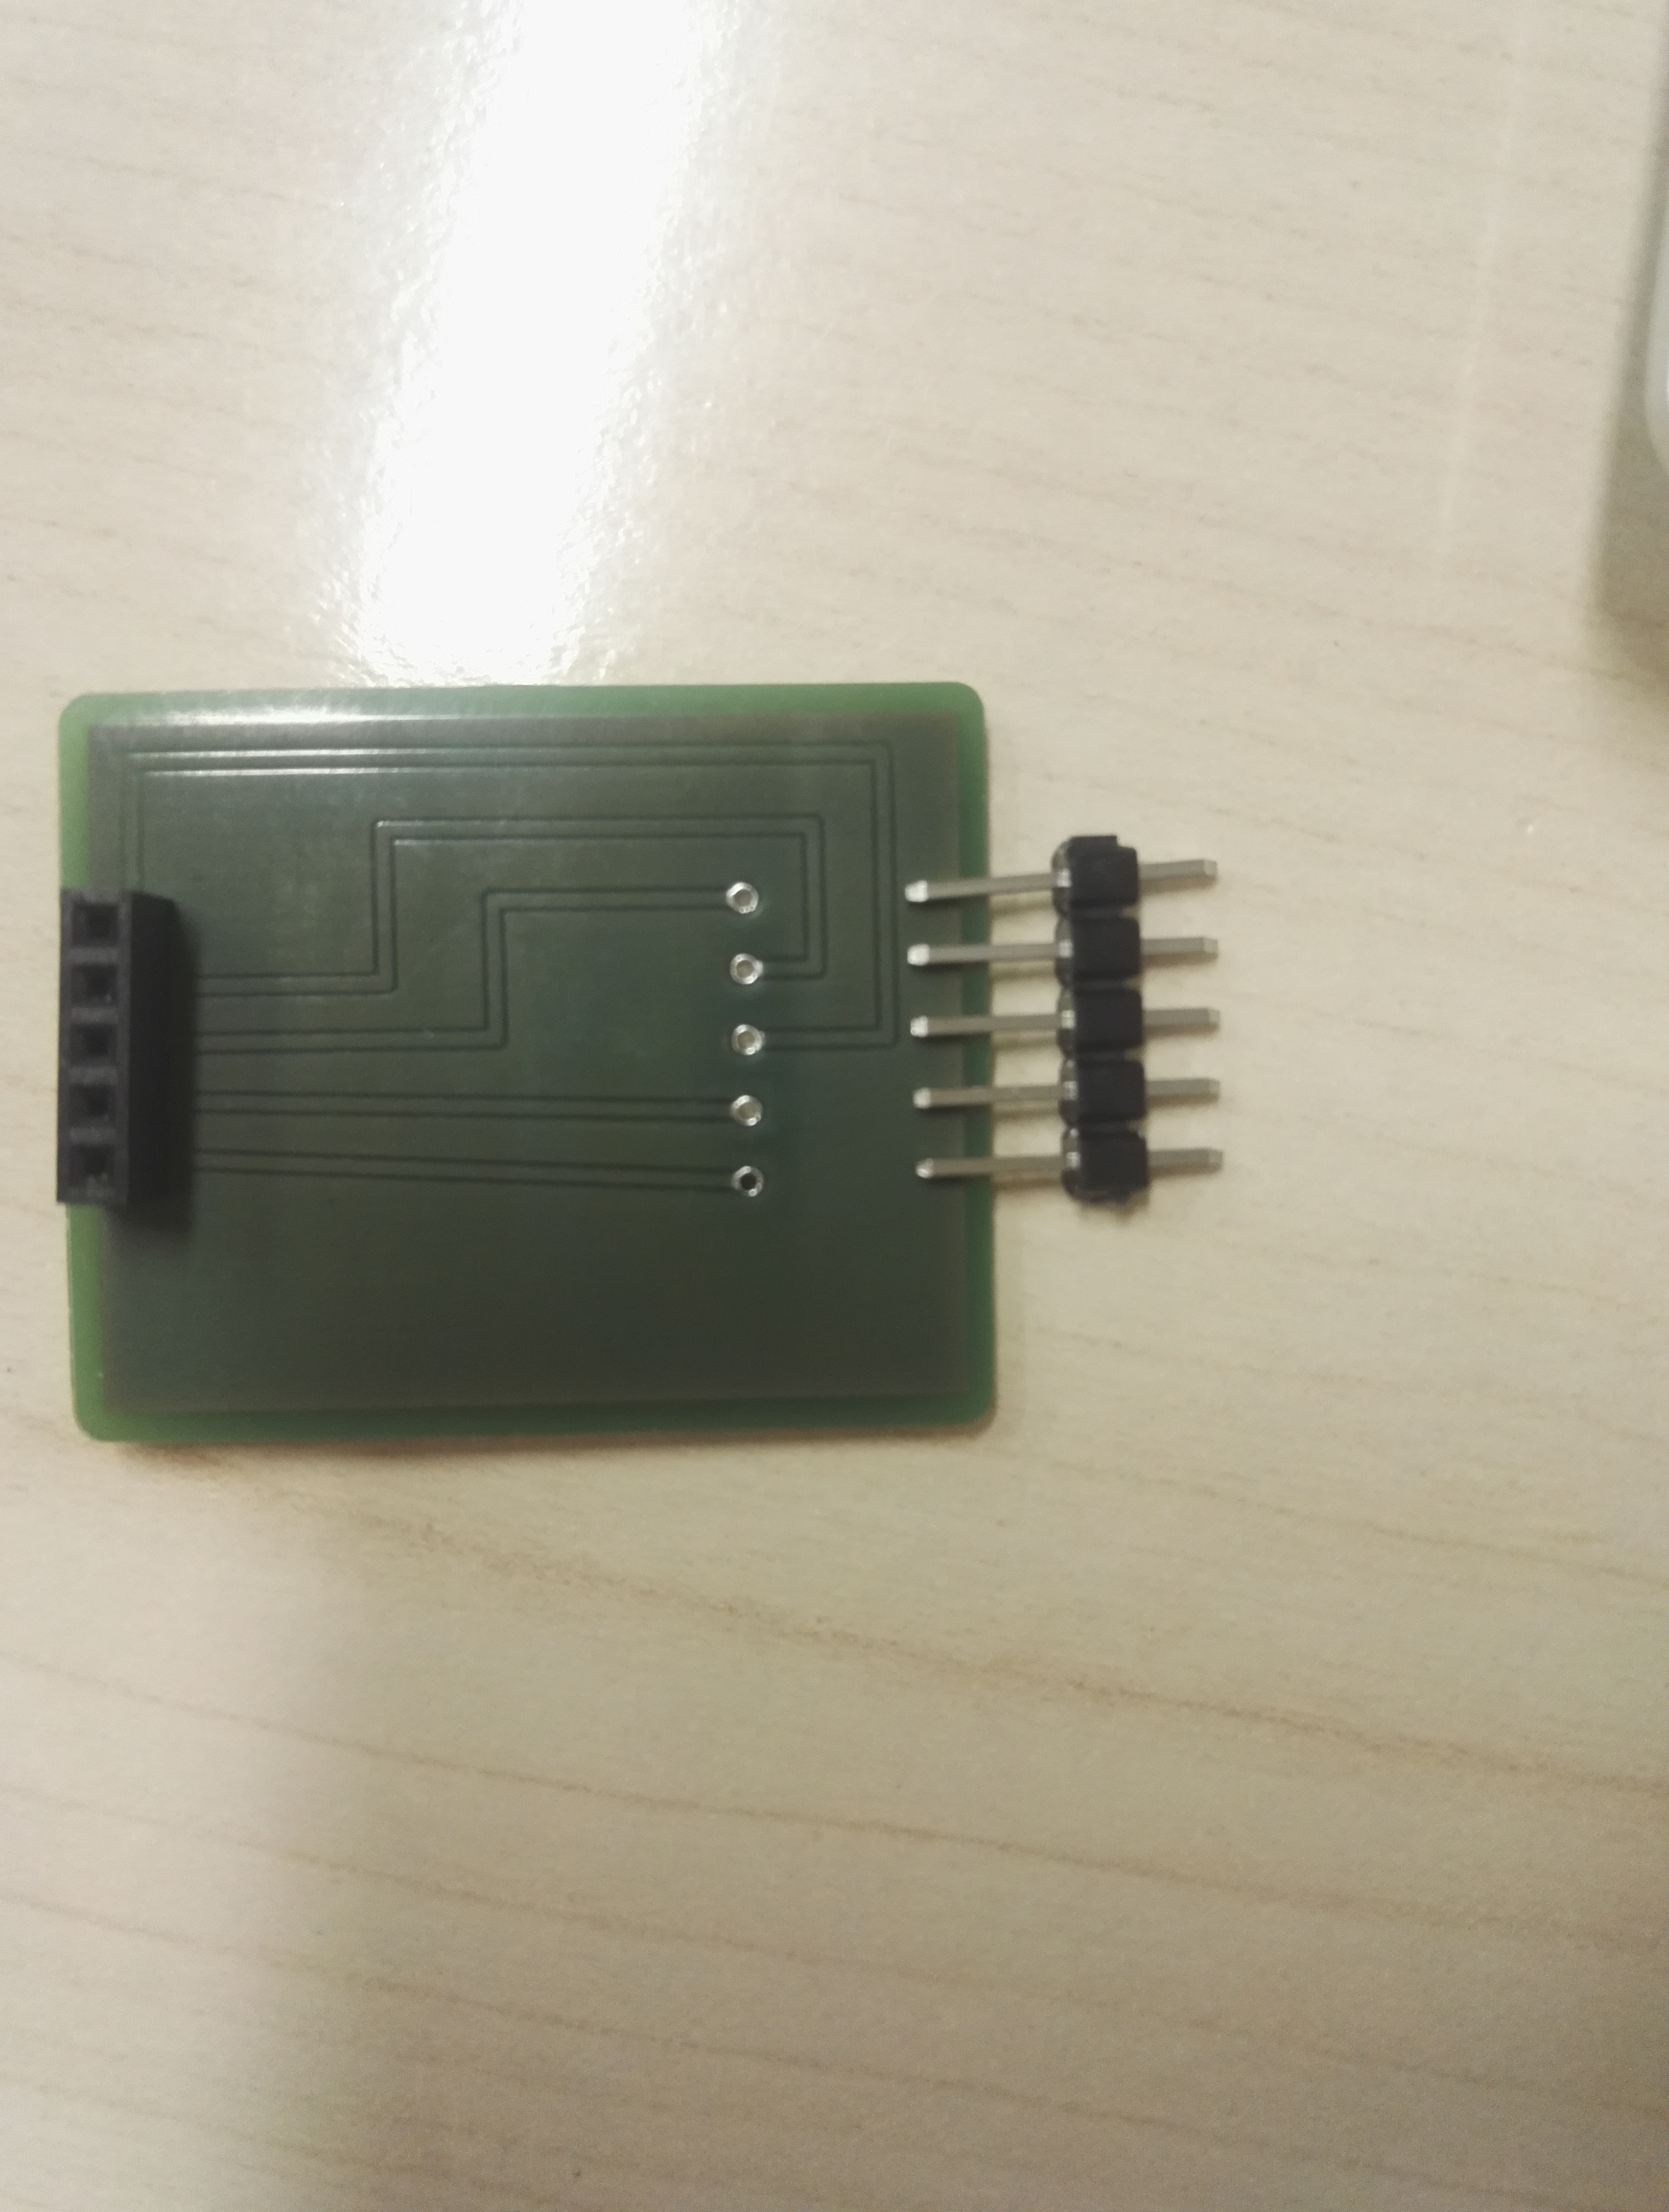
\includegraphics[scale=0.05]{Adapter2.jpg}
\end{center}
\caption{Adaptateur Hbeacon vers MiniProg3}
\label{Adaptateur Hbeacon vers MiniProg3}
\end{figure}

\paragraph{}
Il n'est pas possible de connecter le HBeacon à un ordinateur via un cable usb lambda ou une carte SD, un adaptateur MiniProg3 est nécessaire. La connectique de la carte étant placé dans un ordre différent de celle de l'adaptateur, une carte électronique faisant office d'adaptateur était nécessaire pour simplifier la connexion et éviter les fils. 
Ma mission tout d'abord fut la prise en main du logiciel Eagle, un logiciel de conception de circuit imprimé. Aidé par Arthur, il m'a fallut une journée pour prendre en main le logiciel. 
L'objectif de ma mission consistait en la conception d'une carte adaptateur fonctionnelle permettant de connecter le HBeacon au MiniProg3. Pour ce faire, 5 trous et via de chaque coté de la carte pour les 5 connecteurs du Hbeacon et du MiniProg3 devaient être reliés via des pistes sur le coté cuivre de la carte. Il me fallait également choisir les connecteurs à pins a insérer dans ces trous : mâle/femelle d'un coté, et mâle/mâle de l'autre. Pour concevoir la carte, de nombreuses contraintes devaient être respectées : diamètre des trous et via suivants le connecteur choisi, largeur des pistes, espaces entre les vias suivant l'espaces entre les pins du connecteur choisi, taille de la carte ou encore la sérigraphie. N'ayant aucune expérience avec ce genre de logiciel, la carte paraissant plutôt simple à concevoir sur le papier ne s'est pas faite sans difficulté, notamment pour la gestion des couches (avec une utilisation particulière pour chacune), ou encore pour relier les vias ensembles via les pistes. Le résultat final est visible en figure \ref{Adaptateur Hbeacon vers MiniProg3 sous Eagle}. 
Une fois la carte manufacturée et les connecteurs reçues, il restait simplement à souder les 5 pins de chaque connecteurs dans les 5 trous de la carte. L'adaptateur final fonctionnel est présent en figure \ref{Adaptateur Hbeacon vers MiniProg3}.

Cette première expérience technique m'a permis d'apprendre à utiliser le logiciel Eagle afin d'obtenir un résultat concret et fonctionnel. Le coût de production d'une carte à l'unité étant très cher, il me fallait être rigoureux dans mon travail pour être productif. J'ai également pu mettre en application des connaissances théoriques et pratiques vues à l'école, notamment en électronique : l'utilisation de logiciel de simulation de circuit comme ISIS Proteus ou encore Pspice m'a permis d'être plus à l'aise sur Eagle, logiciel nécessitant un schéma électrique du circuit en amont avant de passer à la carte en elle même. La soudure des pins sur la carte était également un travail minutieux car très proches les unes des autres. 

	\section{Mesures expérimentales de la technologie StimCom}

Le signal StimCom est dérivé de la technologie Stimshop : sa portée est supérieure et il peut envoyer plus d'informations. Stimcom est actuellement utilisé pour le Projet Gravelines, consistant à la communication en interne de la centrale nucléaire de Gravelines. En effet, les ondes radios pouvant poser plusieurs problèmes dans les centrales nucléaire, les ultrasons sont une fin a la communication. 
Ma mission était de réaliser une série de mesures de puissance sonore du signal StimCom (en dB) émis depuis une valise RDK (utilisée pour le projet Gravelines). J'ai donc réalisé ces mesures à l'aide d'un sonomètre et noté les résultats selon la puissance du signal (un potentiomètre permet d'amplifier le signal) afin de dresser un rapport à Arthur. 
Cette missions ne nécessitait aucune compétence en particulier mais il est toujours intéressant de connaitre le fonctionnement de la valise RDK et de la technologie StimCom. Cela m'a également appris à rédiger un rapport résumant les mesures effectuées. 

	\section{Etude et modifications de code en C} 

Afin de générer un signal Stimshop au format .wav, un programme codé en langage C est nécessaire. Ce programme permet notamment de créer un signal d'une minute en saisissant la fréquence souhaitée et les caractères hexadécimaux a envoyer en paramètre. Pour information, le signal Stimshop utilise plusieurs canaux de fréquence qui s'étendent de 17kHz à 21kHz et il peut envoyer jusqu'à 5 caractères hexadécimaux.  
Ma première mission consistait à analyser ce code afin générer un fichier audio .wav puis le visualiser. Les bases en langages C acquises a l'école furent très utiles pour l'étude de ce programme, mais il m'a fallut un certain temps avant de le comprendre dans son intégralité. En effet, certains aspects assez techniques m'ont poussé a poser plusieurs questions à Arthur, mon maître de stage, notamment concernant le fenêtrage du signal. Pour comprendre ce programme, il m'a fallut analyser minutieusement chaque variable de chaque sous programme pour en comprendre la logique. 

\paragraph{}



\begin{figure}[h!]
\begin{center}
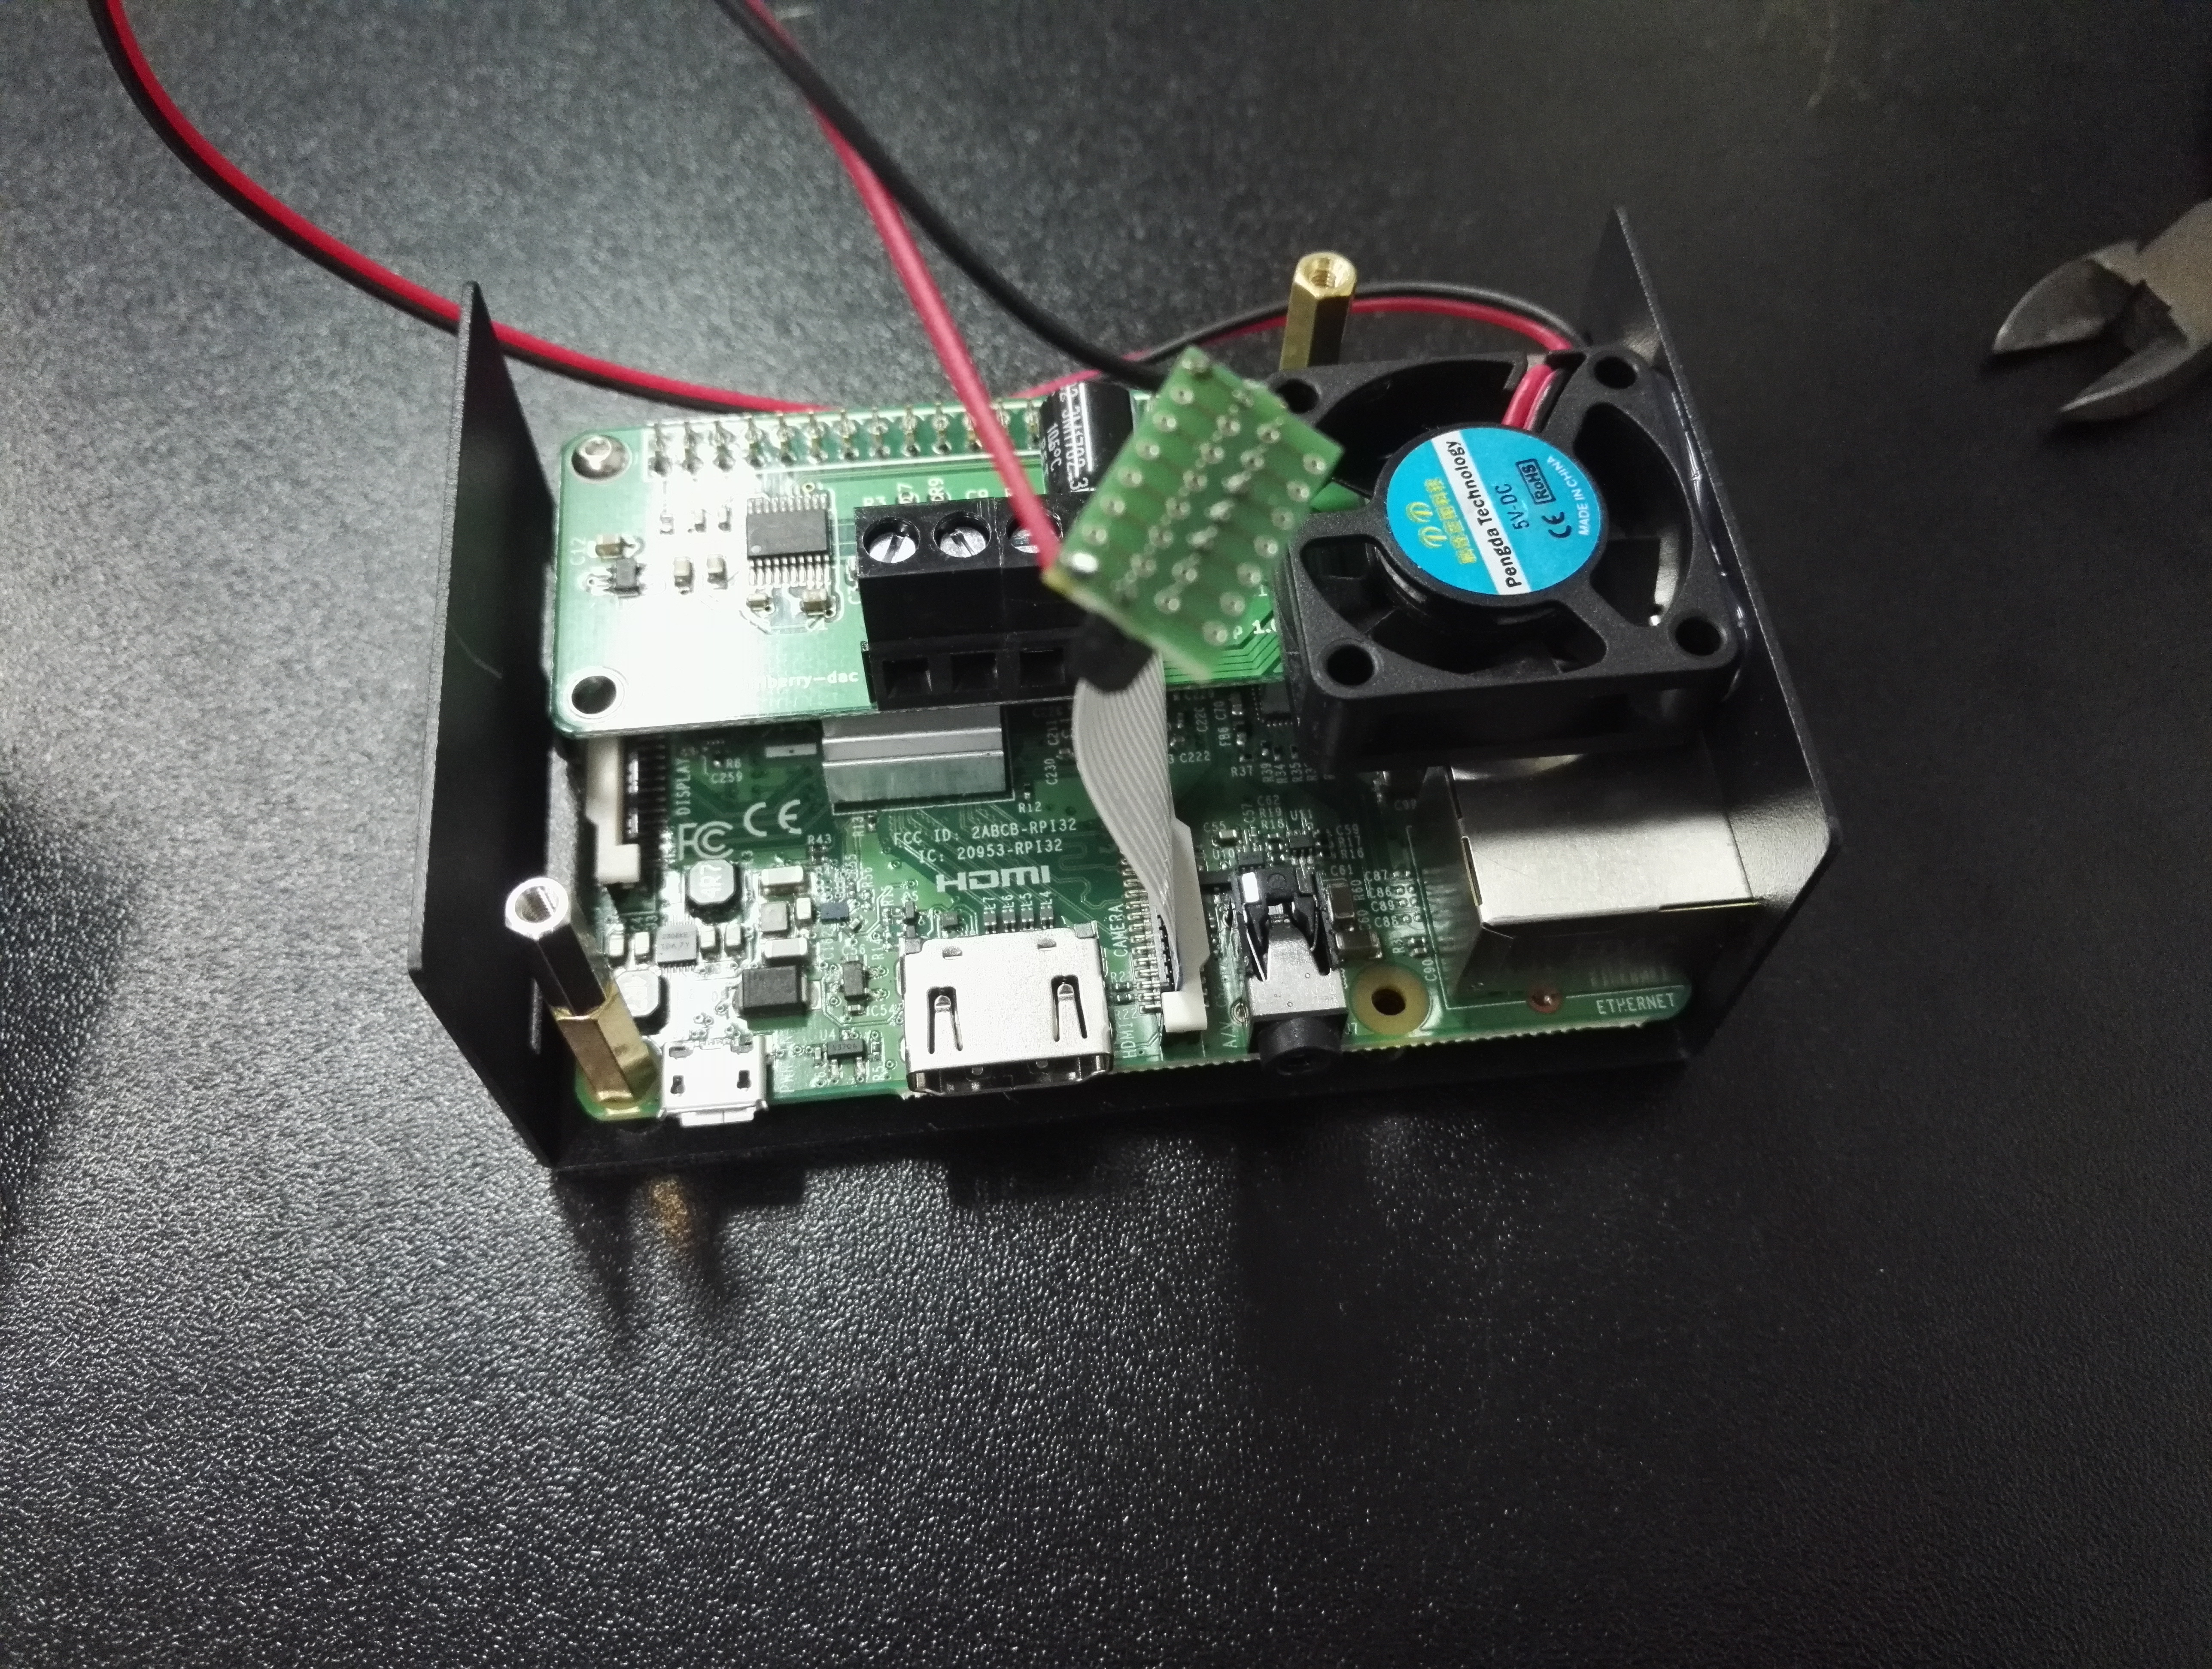
\includegraphics[scale=0.07]{Umix.jpg}
\end{center}
\caption{Interieur d'un boitier Umix}
\label{Interieur d'un boitier Umix}
\end{figure}


\chapter{Réflexions et critiques du monde du travail}
\chapter*{Conclusion}

\end{document}
